\uuid{2Ohs}
\exo7id{7091}
\titre{exo7 7091}
\auteur{megy}
\organisation{exo7}
\datecreate{2017-01-21}
\isIndication{false}
\isCorrection{false}
\chapitre{Géométrie affine euclidienne}
\sousChapitre{Géométrie affine euclidienne du plan}
\module{Géométrie}
\niveau{L2}
\difficulte{}

\contenu{
\texte{
% homothéties
%(\cite[I, prop. 17]{Euclide})
 On donne un cercle  $\mathcal C$ (de centre $O$), un point $M$ à l'extérieur du cercle, les deux tangentes $\mathcal D$ et $\mathcal D'$ à $\mathcal C$ passant par $M$. On notera $A$ et $B$ les points de tangence. 

Le cercle $\mathcal C$ coupe $(MO)$ en deux points $P$ et $Q$. D'autre part, soit $H$ l'intersection de la corde $[AB]$ avec $(OM)$. À l'aide d'homothéties, montrer que les cercles de centres $P$ et $Q$ et passant par $H$ sont tangents à $\mathcal D$ et $\mathcal D'$. 
\begin{center}
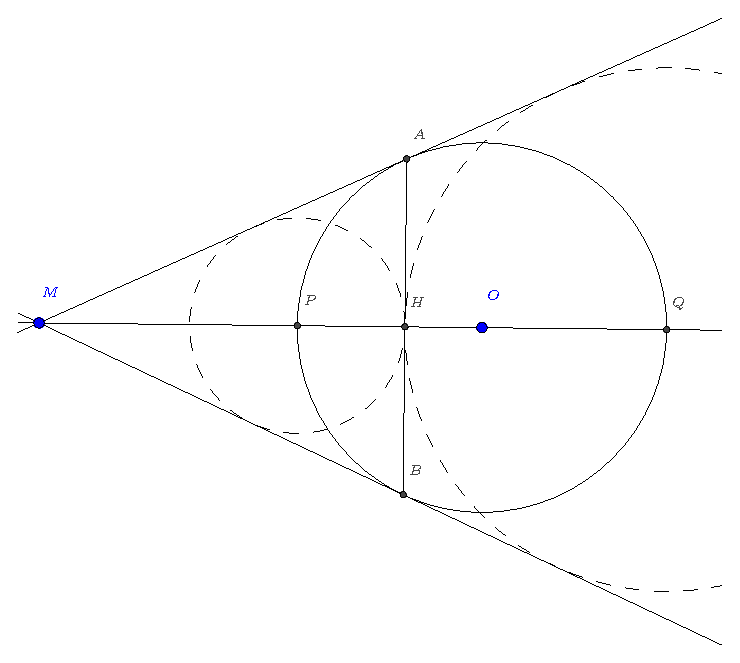
\includegraphics{../images/2Ohs-1}
\end{center}
}
}
